\section{Semantic Modeling of Computational Resources}
\label{sec:semantic}

%\feedback{@Oscar: (following paragraph) this paragraph is actually summarizing and taking for granted many assumptions and preexisting knowledge. Expand it}

%--Deleted base on oscar's feedback
%Scientific workflows are also used for preserving and sharing scientific experiments in science. 


%Some previous research efforts have focused on describing the workflow structure and the 
%experimental data, both input data and results. 

In this work, we argue that in order to achieve reproducibility of a scientific workflow, enough information 
about the computational resources should be provided. These descriptions allow the target audience, 
usually another computational scientist in the same domain, to better understand the underlying 
components involved in a workflow execution.

We define semantic models for describing the main domains of a 
computational infrastructure, and for defining the taxonomy of concepts and the relationships 
between them. These models describe software components, hardware specifications, 
and computational resources (in the form of VMs). They also capture infrastructure 
dependencies of the workflows (e.g services that must be running, available libraries, etc.).
 
 As a result, this process facilitates experiment's reusability since 
a new experiment, which may reuse parts of the workflow previously modeled, or a reproduction 
of a workflow, would benefit from the infrastructure dependencies already described.

We have identified four main domains of interest for documenting computational scientific 
infrastructures~\cite{wicus} and developed a set of models, one for each domain, 
and an ontology network that defines the inter-domain relations between these models 
(Figure~\ref{fig:wicusrels}):

\begin{figure}[!t]
	\centering
	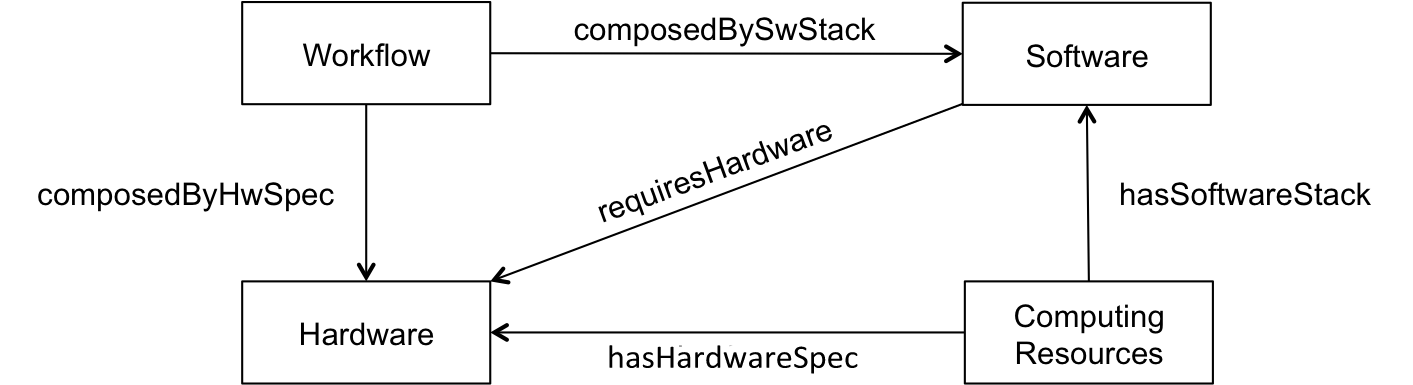
\includegraphics[width=.9\linewidth]{figures/wicusrels}
	\caption{Overview of the ontology network ($\rightarrow$ denotes inter-domain relation).}
	\label{fig:wicusrels}
\end{figure}

\begin{itemize}
	\setlength{\itemsep}{1pt}
	\setlength{\parskip}{0pt}
	\setlength{\parsep}{0pt}

	\item{\emph{Hardware domain}}: it identifies the most common hardware information, 
		including CPU, Storage and RAM memory, and their capacities.
	
	\item{\emph{Software domain}}: it defines the software components involved on the execution. 
    		It includes the pieces of executable software (e.g., scripts, binaries, and libraries) used in 
		the experiment. In addition, dependencies between those components and configuration 
		information are also defined, as well as the required steps for deploying them.
	
	\item{\emph{Workflow domain}}: it describes and relates workflow fragments (a.k.a transformations) 
    		to their dependencies. Therefore, scientists can understand which are the relevant infrastructure 
		components for each part of the workflow.
	
	\item{\emph{Computing Resources domain}}: it expresses the information about the available 
    		computing resources. In this domain, only virtualized resources are currently considered 
		(i.e., virtual machine). It includes the description of the VM image, its provider, and specifications.
\end{itemize}


\rev{The Workflow Infrastructure Conservation Using Semantics ontology 
(WICUS) is an OWL2 (Web Ontology Language) ontology network that 
implements the conceptualization of these domains. This ontology 
network is available online\footnote{http://purl.org/net/wicus} and its goal is to define the relevant and 
required properties for describing scientific computational infrastructures. 
The detailed description of the ontologies, including their main terms and relation
in the context of a workflow execution are provided in~\cite{wicus}.
Currently, two versions of the ontology network have been released. The latest one, released in
August 2014,  includes a set of new properties for better describing software and hardware requirements, 
and also for including the output information of a configuration process (e.g., the resultant IP and port on
which a recently deployed service will be listening).}


\rev{These models have been documented and published online, and have been also aligned with several of well-known vocabularies, such as p-plan\footnote{http://purl.org/net/p-plan} and DCMI Metadata Terms\footnote{http://dublincore.org/documents/dcmi-terms/}. For example, the class wreqs:Workflow that represents a scientific workflow in our domain, has been aligned as a subclass of p-plan:Plan, which in turn is a subclass of prov:Plan, from the PROV vocabulary\footnote{http://www.w3.org/ns/prov}. Further versions of the WICUS ontology network might be aligned with new vocabularies}.  




